\documentclass[a4paper,11pt]{article} %report
%oneside/twoside, openany/openright, twocolumn
\usepackage[T1]{fontenc} % codifica dei font
\usepackage[utf8]{inputenc} % lettere accentate da tastiera
\usepackage[italian]{babel} % lingua del documento
\usepackage{lipsum} % genera testo fittizio
\usepackage{url} % per scrivere gli indirizzi Internet
\usepackage{siunitx}
\usepackage{textcomp}
\usepackage{graphicx}
\usepackage{wrapfig}
\usepackage[final]{pdfpages}
\usepackage[hidelinks]{hyperref} %collegamenti ipertestuali --> \href{ h indirizzo Internet i }{ h testo del collegamento i }


\begin{document}

\author{Fuser Alessandro - VR405372}
\title{Progetto di Software per Sistemi Embedded \\ Graph and SAT problem coloring}
\maketitle

\tableofcontents

\newpage

\section{Obiettivo del Progetto}
Gli obiettivi del progetto assegnato sono:
\begin{enumerate}
	\item Definire una funzione per leggere dei grafi da file, nel formato standard DIMACS;
	\item Usare Espresso per risolvere il problema della colorazione di un grafo;
	\item Usare un SAT solver per risolvere il problema della soddisfacibilità booleana in relazione alla colorazione di un grafo;
	\item Confronto di prestazioni dei due metodi.
\end{enumerate}

\section{Background}
\subsection{Problema della Colorazione di un grafo}
Un grafo è un insieme di elementi detti nodi o vertici che possono essere collegati fra loro da linee chiamate archi o lati o spigoli. Più formalmente, si dice grafo una coppia ordinata G = (V, E) di insiemi, con V insieme dei nodi ed E insieme degli archi, tali che gli elementi di E siano coppie di elementi di V. \\
Il problema della colorazione di un grafo può essere visto come un problema di etichettatura dei vertici del grafo, nel quale è richiesto di assegnare un colore ad ogni vertice, con la condizione che vertici tra loro connessi non abbiano lo stesso colore assegnato. Il problema di k-colorabilità tratta il problema della colorazione di un grafo col vincolo di trovare un numero k il più piccolo possibile tale per cui il grafo possa essere colorato senza violare il vincolo del problema. \\
Una volta trovato il numero di colori k, il problema richiede l'assegnamento di un colore $c_{i}$ con i <= k per ogni vertice $v_{j}$ con j <= $|V|$.\\


\subsection{Problema della soddisfacibilità booleana}
Una formula è in forma normale congiuntiva, indicata anche come CNF (acronimo di Conjunctive Normal Form) se è una congiunzione di clausole, dove le clausole sono una disgiunzione di letterali. Una formula in CNF ha quindi la seguente struttura:

${\displaystyle \bigwedge _{i=1}^{n}\left(\bigvee _{k=1}^{m(i)}L_{i,k}\right)}$ \\

nel quale:
\begin{itemize}
	\item n è il numero di clausole;
	\item m(i) è il numero di letterali della clausola i-esima;
	\item $L_{i,k}$ è il k-esimo letterale della i-esima clausola.
\end{itemize}
Un letterale può essere una variabile booleana (cioè può valere solo 0 o 1, ossia vero o falso) o la negazione di una variabile.\\
Formalmente, la soddisfacibilità booleana, o soddisfacibilità proposizionale o SAT, è il problema di determinare se una formula booleana è soddisfacibile o insoddisfacibile. La formula si dice soddisfacibile se le variabili possono essere assegnate in modo che la formula assuma il valore di verità vero. Viceversa, si dice insoddisfacibile se tale assegnamento non esiste (pertanto, la funzione espressa dalla formula è identicamente falsa).

\subsection{Da k-graph a k-SAT}
Ma come si passa da un problema di colorabilità di un grafo ad un problema di soddisfacibilità booleana?\\
Una volta che si è trovato un numero k tale per cui il grafo è colorabile, la conversione viene effettuata seguendo tali regole:
\begin{enumerate}
	\item Per tutti i vertici, si crea la possibilità che abbia un colore da 1 a k;
	\item Per tutti i vertici, si nega la possibilità che lo stesso vertice possa avere più di un colore;
	\item In funzione degli archi, mi assicuro che i vertici toccati da due archi non abbiano mai lo stesso colore.
\end{enumerate}
\begin{figure}[h]
	\centering
    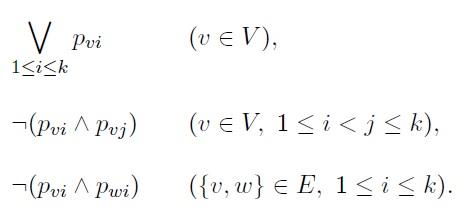
\includegraphics[scale=0.5]{kcolor_to_sat.jpg}
    \caption{Regole riduzione da k-Color a SAT; si definisce $p_{vi}$ il vertice v con il colore i }
\end{figure}
Un esempio di conversione, avendo un grafo a 3 vertici, 2 archi e k = 2, dove il vertice 1 è collegato al vertice 2 ed al vertice 3 é: \newline
$(p_{11} \bigvee p_{12}) \bigwedge (p_{21} \bigvee p_{22}) \bigwedge (p_{31} \bigvee p_{32}) \bigwedge \lnot(p_{11} \bigwedge p_{21}) \bigwedge \lnot(p_{12} \bigwedge p_{22}) \bigwedge \lnot(p_{11} \bigwedge p_{31}) \bigwedge \lnot(p_{12} \bigwedge p_{32})$
\pagebreak
\section{Formato DIMACS}
Il formato scelto per i grafi è lo standard DIMACS edge, nel quale:
\begin{itemize}
	\item Le righe che iniziano con "c" sono dei commenti per spiegare il grafo;
	\item La riga che inizia con "p" indica il numero di nodi e di archi;
	\item Le righe che iniziano con "e" indicano il collegamento tra due vertici.
\end{itemize}
Esempio di grafo DIMACS:\\
\begin{verbatim}
c FILE: myciel3.col
c SOURCE: Michael Trick (trick@cmu.edu)
c DESCRIPTION: Graph based on Mycielski transformation. 
c              Triangle free (clique number 2) but increasing
c              coloring number
p edge 11 20
e 1 2
e 1 4
e 1 7
e 1 9
e 2 3
e 2 6
e 2 8
e 3 5
e 3 7
e 3 10
e 4 5
e 4 6
e 4 10
e 5 8
e 5 9
e 6 11
e 7 11
e 8 11
e 9 11
e 10 11
\end{verbatim}
\begin{figure}
	\centering
	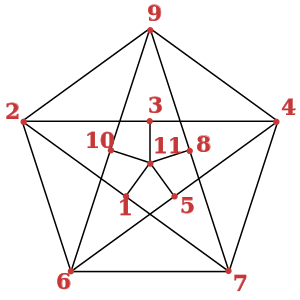
\includegraphics[scale=0.5]{myciel.jpg}
	\caption{Rappresentazione del grafo myciel3}
\end{figure}
Il formato scelto per la rappresentazione delle formule CNF è lo standard DIMACS cnf, dove:
\begin{itemize}
	\item La prima riga, che comincia con "p", indica che il formato è in CNF ed il numero di variabili e clausole;
	\item Le righe successive indicano le clausole ed ogni riga termina con uno zero; un numero rappresenta una variabile e, se preceduta da un -, allora tale variabile, all'interno della clausola, è negata.
\end{itemize}

\section{Colorabilità del grafo tramite espresso}

Dato un generico grafo G(V, E), con V l’insieme dei nodi e E l’insieme dei vertici, costruiamo in funzione delle
sottoregioni presenti nel grafo, un PLA nel modo seguente:
\begin{itemize}
	\item Il numero delle variabili di input è uguale al numero dei nodi $|V|$ presenti nel grafo;
	\item Restituiamo in output 1 bit che indicherà la colorabilità della sottoregione;
	\item Costruiamo il PLA di tipo fr, pertanto il significato dei termini è il seguente:
	\begin{itemize}
		\item con il termine 1, indichiamo che il prodotto dei termini appartenenti all’insieme ON-Set;
		\item con il termine 0, indichiamo che il prodotto dei termini appartenenti all’insieme OFF-Set;
		\item con il termine -, indichiamo l’insieme DC-Set, il quale rappresenta il complemento dell’unione tra ON-Set e OFF-Set;
	\end{itemize}
	\item Definiamo l’insieme degli ON-Set, come $|V|$ righe che rappresentano le aree della mappa che possono avere il medesimo colore;
	\item Definiamo l’insieme degli OFF-Set, pari al numero degli archi contenuti in E, come l’insieme delle regioni
	che devono avere colore differenti.
\end{itemize}
Esempio di trasformazione, prendendo il grafo presentato prima:
\begin{verbatim}
.i 11
.o 1
.type fr
-0000000000 1
0-000000000 1
00-00000000 1
000-0000000 1
0000-000000 1
00000-00000 1
000000-0000 1
0000000-000 1
00000000-00 1
000000000-0 1
0000000000- 1
11--------- 0
1--1------- 0
1-----1---- 0
1-------1-- 0
-11-------- 0
-1---1----- 0
-1-----1--- 0
--1-1------ 0
--1---1---- 0
--1------1- 0
---11------ 0
---1-1----- 0
---1-----1- 0
----1--1--- 0
----1---1-- 0
-----1----1 0
------1---1 0
-------1--1 0
--------1-1 0
---------11 0
.end
\end{verbatim}

\pagebreak

\section{Soddisfacibilità CNF}

\subsection{Conversione e soluzione}
Dato il grafo generico G=(V,E), è possibile effettuare la conversione in formato DIMACS cnf, descritto sopra, tramite le regole presentate. Ma come trovo il numero di colori per effettuare tale conversione?
Due sono gli approcci presentati, entrambi basati sul problema Clique, ossia un insieme di vertici di V tale che esiste un arco tra tutti i vertici dell'insieme, per cui, nel nostro problema, corrisponde al limite minimo di colori in quanto vertici collegati devono avere colori diversi:
\begin{enumerate}
	\item Algoritmo di ricerca binaria, che comincia usando un k massimo (=$|V|$), un minimo dato dalla dimensione massima della clique e, ogni volta che la formula è soddisfacibile con tale k, ripete il problema con un k dimezzato, fino a che la formula non è più soddisfacibile ed allora aumenta k di un valore a metà tra l'ultimo soddisfacibile e quello attuale;
	\item sfruttando il problema della Clique, trovo quella più grande, che mi rappresenta il lower bound di colori e da questo aumento k di 1 fino a che la formula non è soddisfacibile.
\end{enumerate}
Il metodo che è stato utilizzato per la conversione è il secondo, in quanto si è dimostrato più veloce in tutte le situazioni.
Una volta scelto un k, la conversione viene effettuata nel formato DIMACS cnf, presentato precedentemente. Per l'esempio presentato prima, la conversione con 4 colori è:
\begin{verbatim}
p cnf 44 91
1 2 3 4 0
5 6 7 8 0
9 10 11 12 0
13 14 15 16 0
17 18 19 20 0
21 22 23 24 0
25 26 27 28 0
29 30 31 32 0
33 34 35 36 0
37 38 39 40 0
41 42 43 44 0
-1 -5 0
-2 -6 0
-3 -7 0
-4 -8 0
-1 -13 0
-2 -14 0
-3 -15 0
-4 -16 0
-1 -25 0
-2 -26 0
-3 -27 0
-4 -28 0
-1 -33 0
-2 -34 0
-3 -35 0
-4 -36 0
-5 -9 0
-6 -10 0
-7 -11 0
-8 -12 0
-5 -21 0
-6 -22 0
-7 -23 0
-8 -24 0
-5 -29 0
-6 -30 0
-7 -31 0
-8 -32 0
-9 -17 0
-10 -18 0
-11 -19 0
-12 -20 0
-9 -25 0
-10 -26 0
-11 -27 0
-12 -28 0
-9 -37 0
-10 -38 0
-11 -39 0
-12 -40 0
-13 -17 0
-14 -18 0
-15 -19 0
-16 -20 0
-13 -21 0
-14 -22 0
-15 -23 0
-16 -24 0
-13 -37 0
-14 -38 0
-15 -39 0
-16 -40 0
-17 -29 0
-18 -30 0
-19 -31 0
-20 -32 0
-17 -33 0
-18 -34 0
-19 -35 0
-20 -36 0
-21 -41 0
-22 -42 0
-23 -43 0
-24 -44 0
-25 -41 0
-26 -42 0
-27 -43 0
-28 -44 0
-29 -41 0
-30 -42 0
-31 -43 0
-32 -44 0
-33 -41 0
-34 -42 0
-35 -43 0
-36 -44 0
-37 -41 0
-38 -42 0
-39 -43 0
-40 -44 0
\end{verbatim}


La risoluzione tramite MINISAT porta al seguente assegnamento:\\
SAT
-1 -2 -3 4 5 -6 -7 -8 -9 -10 11 -12 -13 -14 15 -16 17 -18 -19 -20 -21 22 -23 -24 -25 26 -27 -28 -29 30 -31 -32 -33 34 -35 -36 -37 38 -39 -40 41 -42 -43 -44 0\\
Dove SAT indica che la formula è soddisfacibile tramite l'assegnamento delle variabili indicato precedentemente, dove se ho un "-" allora la variabile è posta a FALSE, altrimenti a TRUE e lo zero indica la fine del file.

\pagebreak

\section{Prestazioni}
Tutte le prove sono state fatto su una macchina portatile con un i7-4710HQ e 16GB di RAM.\\
Il confronto è stato fatto su una serie di grafi presi dal sito \href{https://sites.google.com/site/graphcoloring/vertex-coloring}{Graph Coloring Benchmarks}. Sono stati relazionati i tempi relativi alla soluzione con Espresso, con Minisat \cite{minisat} (solutore per SAT), DPLL \cite{dpll}(solutore per SAT) e i risultati della \cite{tesi}.
Per ogni problema, è stato impostato un timer di 30 minuti in quanto eravamo interessati ad una risoluzione veloce del problema. L'unica eccezione viene data dal problema \href{https://it.wikipedia.org/wiki/Rompicapo_delle_otto_regine}{\textbf{queen8}}, che viene preso come esempio principale della difficoltà computazionale.
Le tempistiche sono riassunte nella tabella successiva, dove:
\begin{itemize}
	\item La prima colonna riporta il nome del problema;
	\item La seconda colonna riporta il numero di vertici del grafo;
	\item La terza colonna riporta il numero di archi del grafo;
	\item La quarta colonna riporta la densità del grafo;
	\item La quinta colonna riporta il limite inferiore della dimensione della clique massima possibile;
	\item La sesta colonna riporta la dimensione della clique di dimensione massima trovata;
	\item La settima colonna riporta il numero cromatico migliore trovato in letteratura;
	\item L'ottava e la nona colonna riportano il numero cromatico ed il tempo, in secondi, usando Espresso;
	\item La decima ed undicesima colonna riportano il numero cromatico ed il tempo, in secondi, usando Minisat, applicando il secondo metodo di conversione descritto, ossia sfruttando il problema della Clique;
	\item La dodicesima colonna riporta il tempo, in secondi, riferito nella \cite{tesi};
	\item Le ultime due colonne riportano il numero cromatico ed il tempo, in secondi, ancora usando Minisat, ma stavolta applicando il primo metodo di conversione, ossia l'algoritmo di ricerca binaria del colore.
\end{itemize}

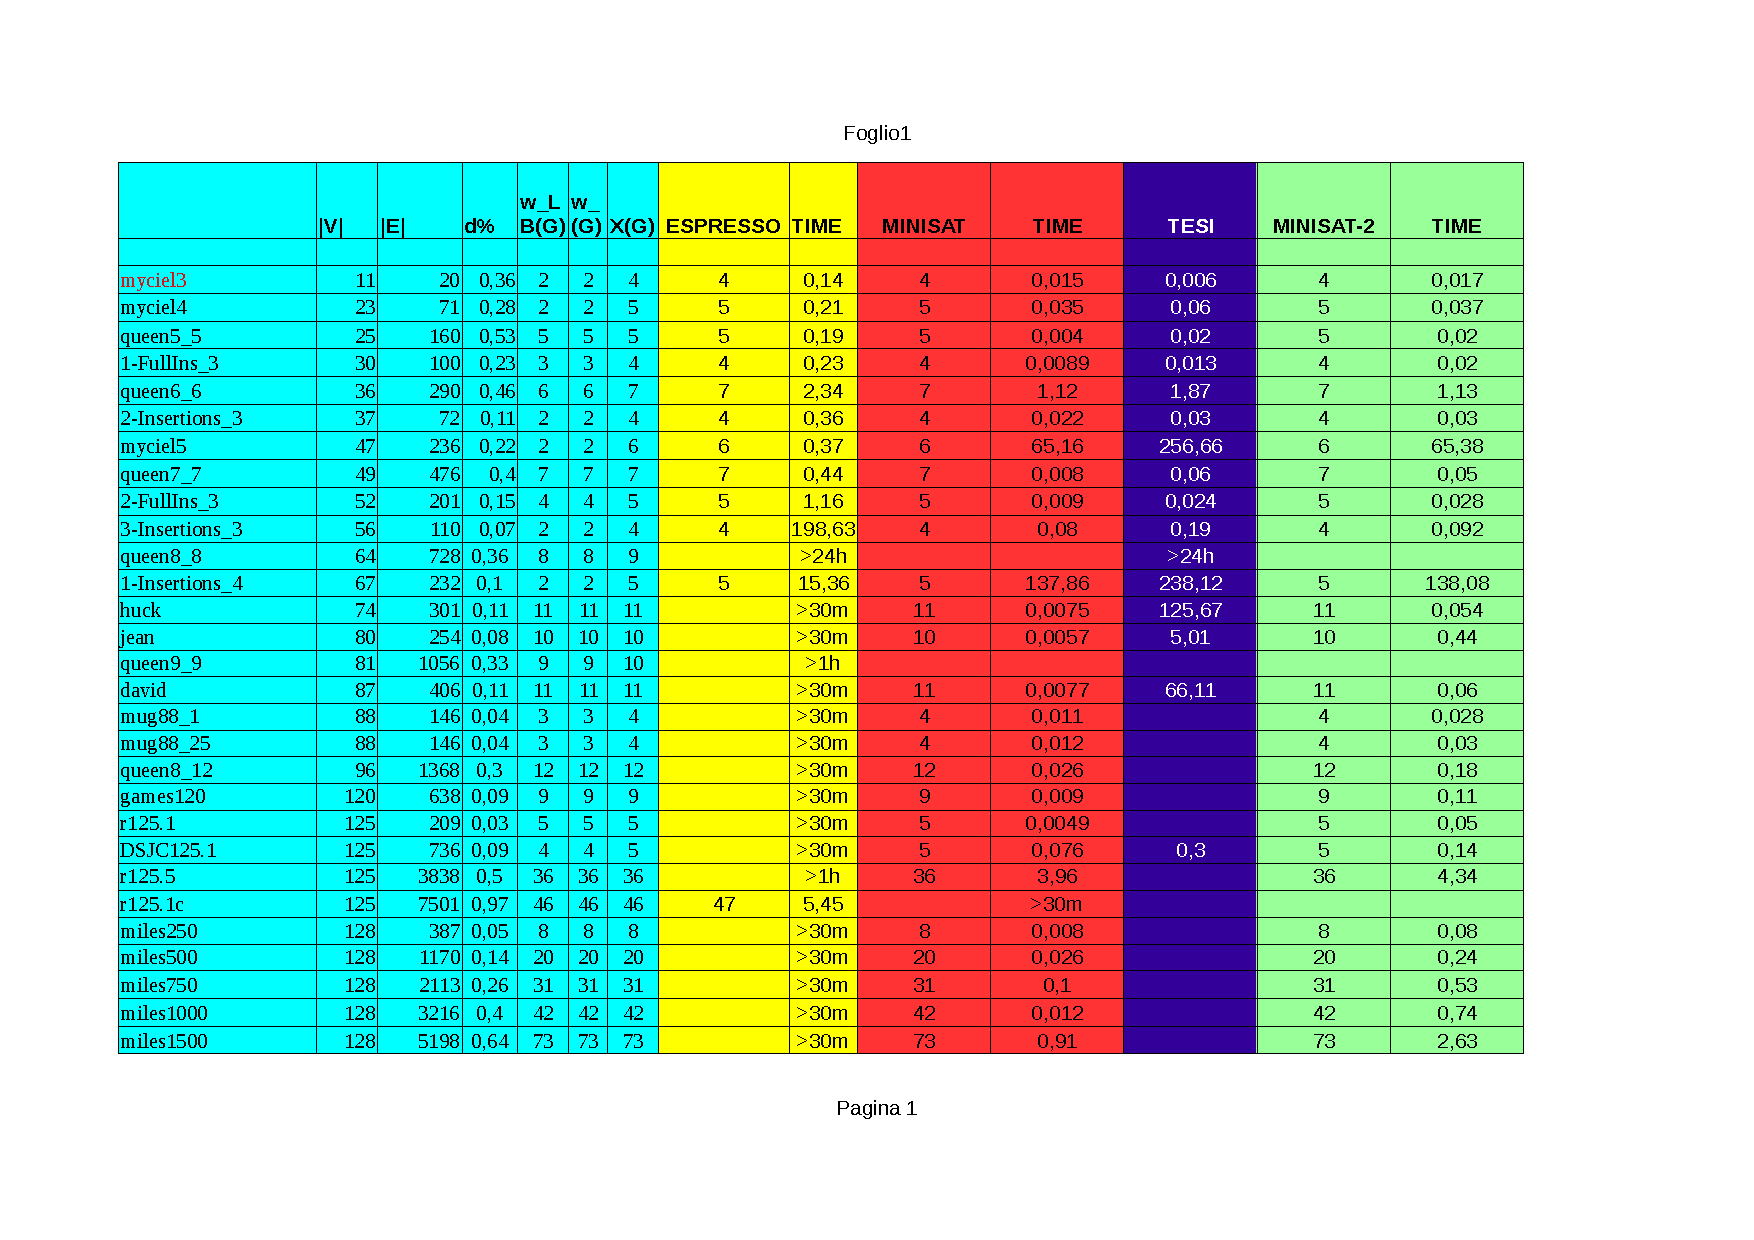
\includepdf[pages=-]{datifile.pdf}

\subsection{Commenti}
Come si può notare, in tutti i problemi la risoluzione tramite MINISAT è molto più rapida rispetto ad Espresso. Questo potrebbe essere dovuto alla complessità computazionale della minimizzazione di espresso, che può essere molto dispendiosa sia in termini di tempo che di risorse, dato che le 3 funzioni interne di espresso portano a colorare il grafo in funzione degli implicanti primi essenziali della funzione di partenza (complessi da calcolare).\\
E' interessante notare però come il problema queen8 (così come il problema queen9) non è stato risolto nè da espresso nè da MINISAT in termini ragionevoli (24 ore), il che ci fa capire che problemi difficili sono tali sia per espresso che per MINISAT.\\
Rispetto al DPLL, MINISAT è più veloce in quanto si basa sullo stesso algoritmo usato per DPLL, ma aggiungendo molte ottimizzazioni, come si legge in \cite{minisat}. DPLL è stato abbandonato dopo pochi problemi in quanto riportano sempre tempi maggiori rispetto a MINISAT, per cui ci si è concentrati sul migliore risolutore per SAT.\\
Un altro aspetto da tenere conto è il fatto che sfruttare il problema della clique come punto di partenza della scelta dei colori è più efficace rispetto ad usare un approccio binario per la ricerca dei colori e la clique come lower bound. Questo è dovuto al fatto che, nella maggior parte dei casi, il valore della clique più grande è molto vicino al numero cromatico del grafo, per cui le iterazioni sono minori.

\pagebreak

\section{Lavori Futuri}
Per lavori futuri, sarebbe interessante provare altri solutori SAT in modo da vedere se anche i problemi che non vengono risolti usando i solutori presentati vengono decisi.\\
Un altro aspetto interessante sarebbe quello di capire se la non risoluzione è dovuta alla semplice mancanza di sufficiente potenza di calcolo, per cui sfruttare un computer dalle prestazioni superiori, magari un supercomputer.\\
Dato che Espresso, nella sua esecuzione, trova tutte le possibili colorazioni del grafo dopo aver definito un determinato k (numero dei colori) ma ne restituisce una sola tra quelle trovate, mentre un qualsiasi algoritmo di risoluzione SAT cerca di risolvere il più in fretta possibile il problema e restituisce la prima colorazione trovata che soddisfa la formula, un'ulteriore tema che potrebbe essere interessante affrontare è quello della multi-colorazione dei grafi, ossia trovare tutte le possibili colorazione del grafo dato il k (numero di colori) e vedere quale di esse è più vantaggiosa usare rispetto ad altre metriche da definire, per cui vedere se anche in questo problema Espresso (che codifica già in modo compatto tutte le soluzioni, ossia trova già tutte le possibili colorazioni) è più lento rispetto ai solutori SAT (che deve ora iterare più volte per trovare tutte le possibili colorazioni).


\pagebreak

\begin{thebibliography}{9}
	\bibitem{tesi} Stefan Kugele,  
	\emph{Efficient Solving of Combinatorial Problems using SAT-Solvers}
	
	\bibitem{minisat} \href{http://minisat.se/}{http://minisat.se/}
\end{thebibliography}


\end{document}